\begin{frame}{nonlinear SVM -- method summary}

\footnotesize

% \maketag{SUPERVISED} 
\maketag{CLASSIFICATION} \maketag[50]{REGRESSION} \maketag{NONPARAMETRIC} 
\maketag{BLACK-BOX}

\medskip

\highlight{General idea}
\begin{itemize}
  \item Move \textbf{beyond linearity} by mapping data to 
  transformed space where they are linearly separable
  \item \textbf{Kernel trick} %\textcolor{blue}{(based on Mercer's theorem,  existence of reproducing kernel Hilbert space)}: 
  \begin{itemize}
    % \item Replace two-step operation feature map $\phi$ $\leadsto$ inner product 
    % by \textbf{kernel} $k: \Xspace \times \Xspace \rightarrow \R$, s.t.
    % $\scp{\phix}{\phixt} = \kxxt$
    \item No need for explicit construction of feature maps
    \item Replace inner product of feature map $\phi$ by \textbf{kernel}: $\scp{\phix}{\phixt} = \kxxt$
  \end{itemize}
  %\item Loss of interpretability through nonlinear feature map
\end{itemize}

\medskip

% \operatorname{sign}(\mathbf{w} \cdot \Phi(\mathbf{x})+b)

\highlight{Hypothesis space} ~~
% $\Hspace = \left \{ \fx = \sumin \alpha_i \yi k(\xi, \xv)  + \theta_0 ~|~
% \theta_0, \alpha_i \in \R ~ \forall i \right \} $
%\textcolor{blue}{$\Hspace = \{ \operatorname{sign}(\sumin \alpha_i \yi k(\xi, \xv)  + \theta_0) |\ (\theta_0, \thetab) \in \R^{p+1} \} $}
$\left \{ \fx = \sumin \alpha_i \yi \langle \phi \left( \xi \right), 
    \phi(\xv) \rangle  + 
    \theta_0 ~|~ \theta_0, \alpha_i \in \R ~ \forall i \right \}$

\begin{minipage}[b]{0.33\textwidth}
  \centering
  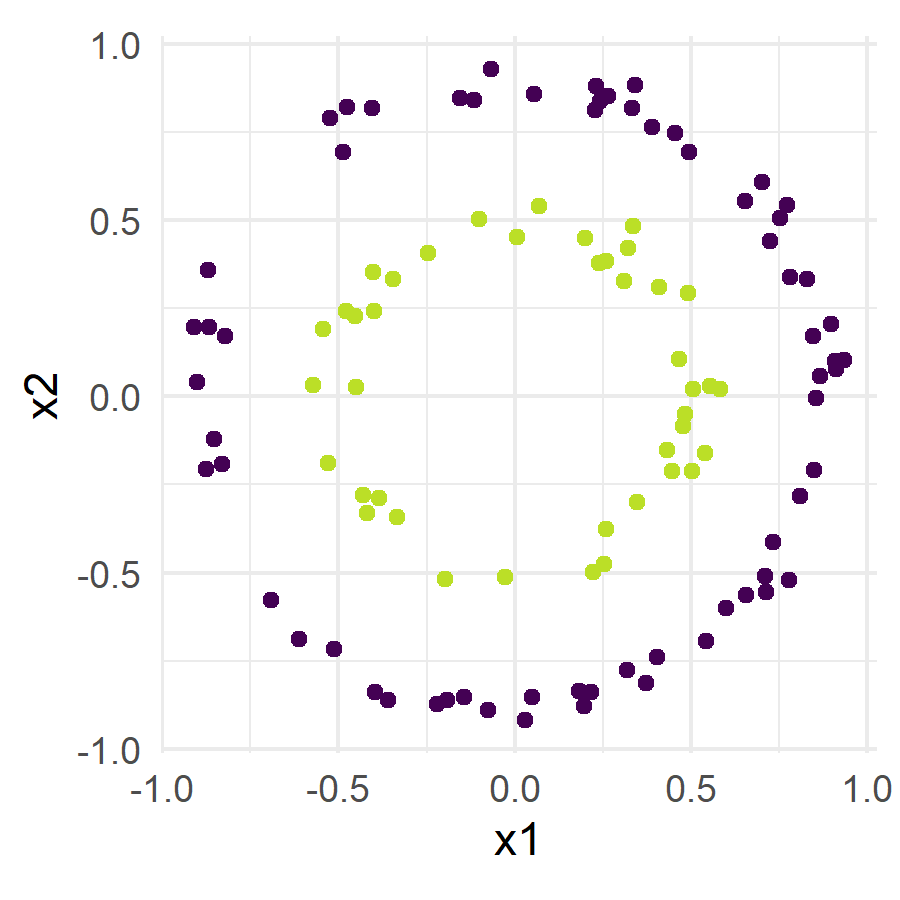
\includegraphics[width=0.5\textwidth]{
  figure/circles_ds.png} \\
  \tiny{Nonlinear problem in original space} 
\end{minipage}
\begin{minipage}[b]{0.66\textwidth}
  \centering
  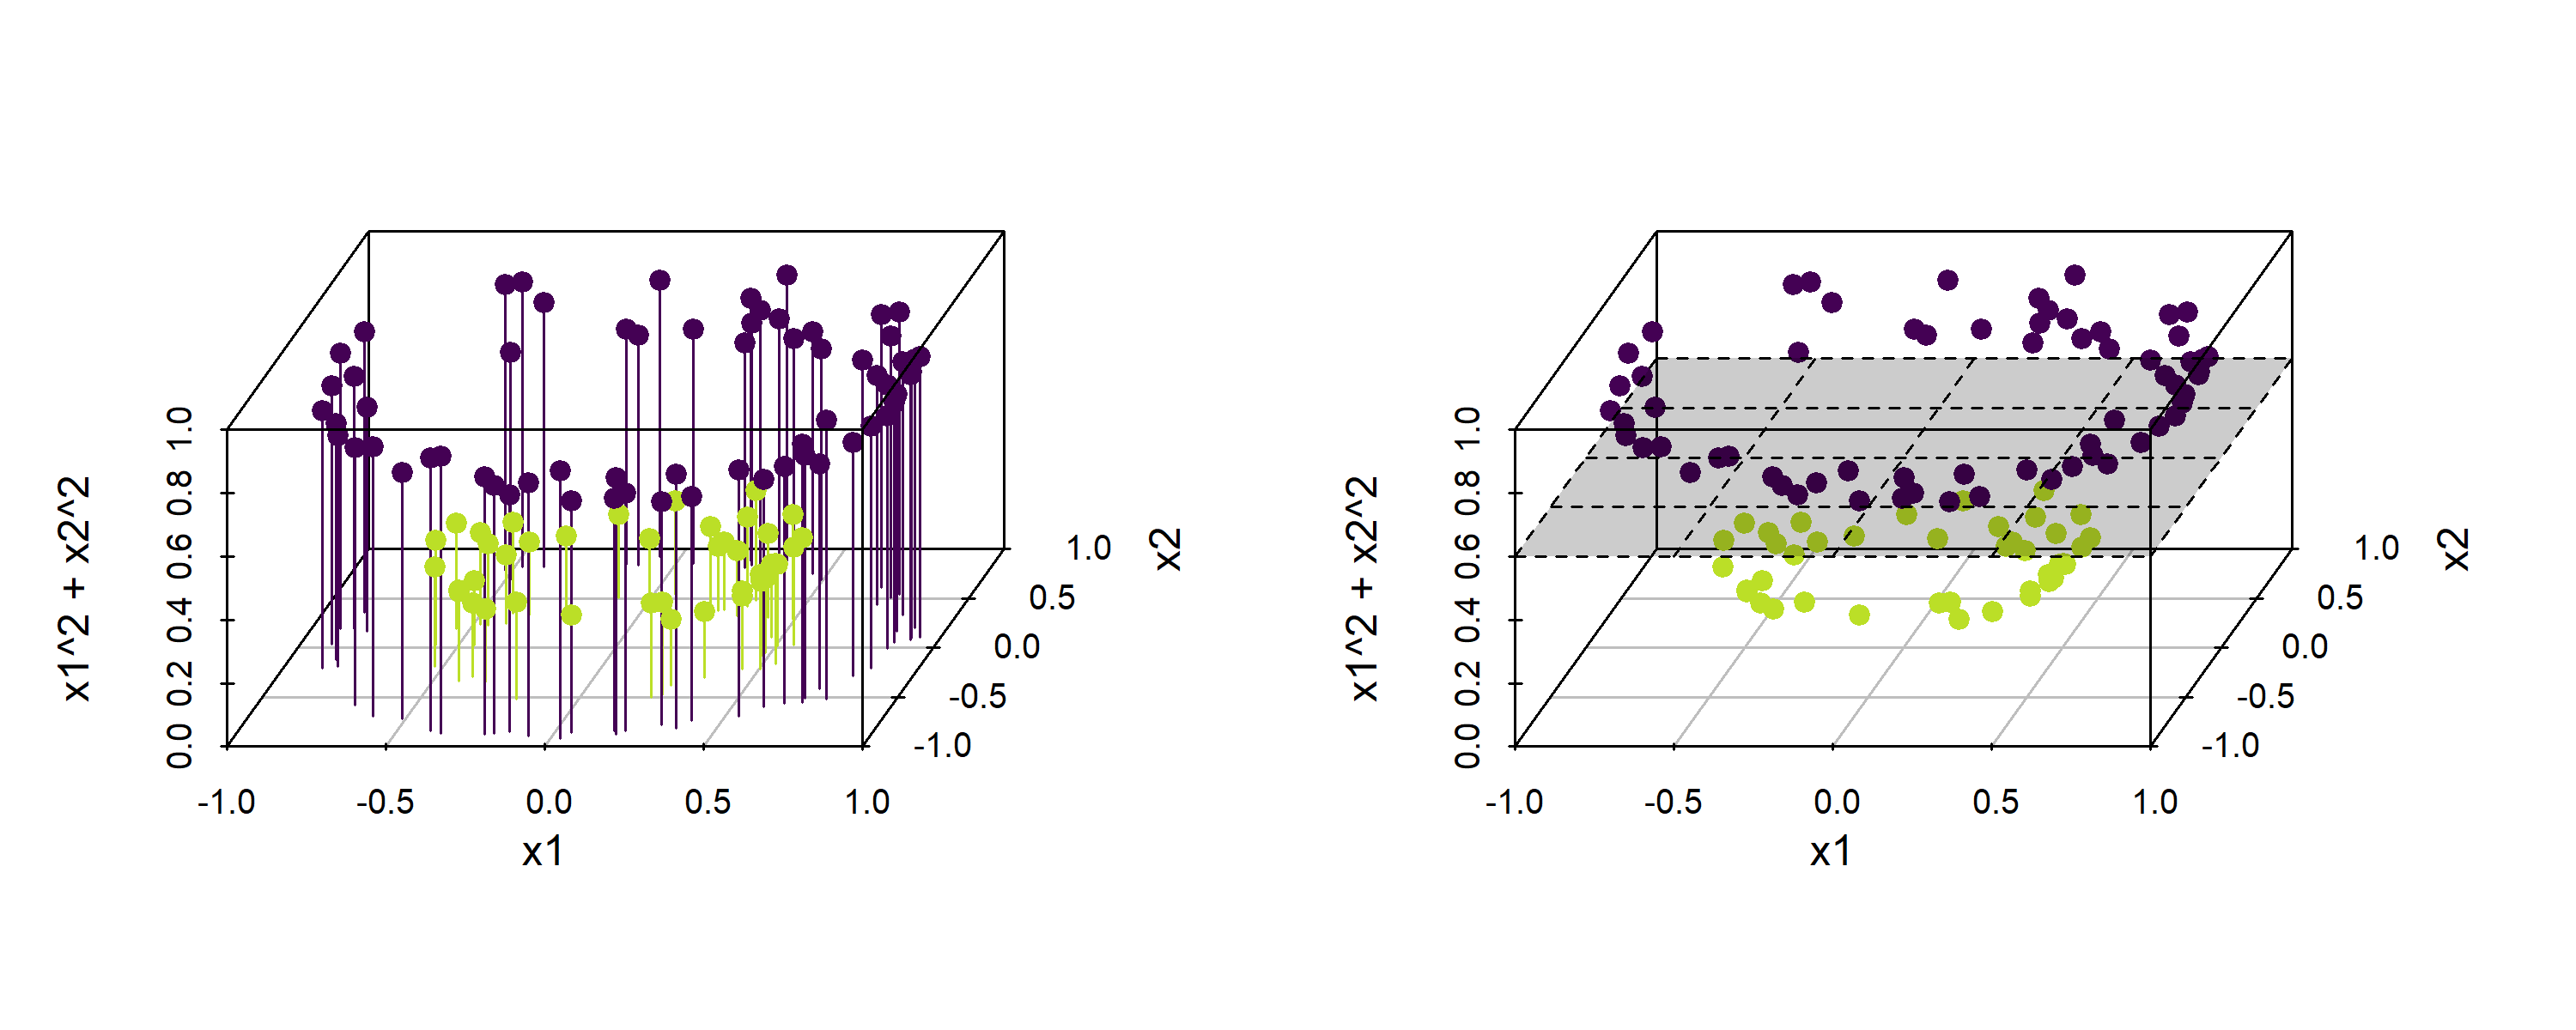
\includegraphics[width=0.9\textwidth, trim=0 30 0 0, clip]{
  figure/circles_feature_map.png} \\
  \tiny{Mapping to 3D space and subsequent linear separation -- implicitly 
  handled by kernel in nonlinear SVM}
\end{minipage}

\end{frame}

% ------------------------------------------------------------------------------

\begin{frame}{nonlinear SVM -- method summary}

\footnotesize

\highlight{Dual problem} ~~ \textbf{Kernelize} dual (soft-margin) SVM problem, 
replacing all inner products by kernels:
$$\max_{\alphav} \sumin \alpha_i - \frac{1}{2}\sumin \sumjn
\alpha_i\alpha_j\yi y^{(j)} \textcolor{blue}{k(\xi, \xi[j])}, ~~ \text{s.t. } ~~ 
0 \le \alpha_i \le C, ~~ \sumin \alpha_i \yi = 0.
$$

\medskip

\highlight{Hyperparameters} ~~ Cost $C$ of margin violations, kernel 
hyperparameters (e.g., width of RBF kernel)

\medskip

\highlight{Interpretation as basis function approach}

\begin{minipage}[c]{0.5\textwidth}

  \begin{itemize}
    \item \textbf{Representer theorem:} dual soft-margin SVM problem expressible 
    through 
    $\thetab = \sumjn \alpha_j \phi \left(\xi[j] \right)$ \\
    \item Sparse, weighted sum of \textbf{basis functions} with $\alpha_j = 0$ 
    for non-SVs
    \item Result: \textbf{local} model with smoothness depending on kernel 
    properties
  \end{itemize}
\end{minipage}
\hfill
\begin{minipage}[c]{0.4\textwidth}
  \centering
  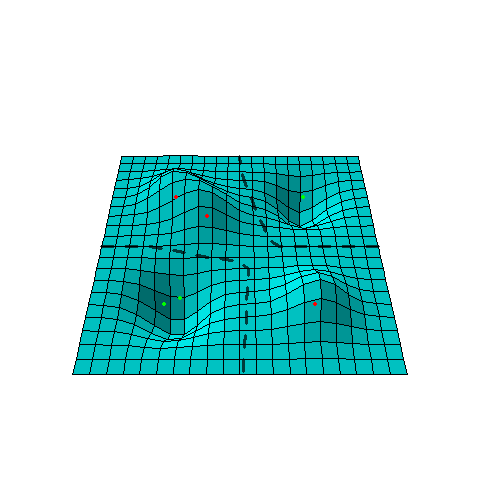
\includegraphics[width=0.9\textwidth, trim=0 70 0 100, clip]{
  figure/svm_rbf_as_basis.png} \\
  \tiny{RBF kernel as mixture of Gaussian basis functions, forming
  bumpy, nonlinear decision surface to discern red and green points}
\end{minipage}

\end{frame}

% ------------------------------------------------------------------------------

\begin{frame}{nonlinear SVM -- Practical hints}

\footnotesize

\highlight{Common kernels}

\begin{itemize}
  \item \textbf{Linear} kernel: dot product of given observations ~~ 
  $\Rightarrow \kxxt = \xv^\top \xtil$ ~~ $\Rightarrow$ linear SVM
  \item \textbf{Polynomial} kernel of degree $d \in \N$: monomials (i.e., 
  feature interactions) up to $d$-th 
  order ~~$\Rightarrow 
  \kxxt = \left(\xv^\top \xtil + b \right)^d, ~ b \geq 0$
  \item \textbf{Radial basis function (RBF)} kernel: infinite-dimensional 
  feature space, allowing for perfect separation of all finite 
  datasets ~~ $\Rightarrow \kxxt = \exp \left( -\gamma \| \xv - \xtil \|_2^2 
  \right )$ with 
  bandwidth parameter $\gamma > 0$
\end{itemize}
 
\medskip

 \highlight{Tuning}
 
 \begin{itemize}
  \item High sensitivity w.r.t. hyperparameters, especially those of kernel
  ~~ $\Rightarrow$ \textbf{tuning} very important
  \item For RBF kernels, use \textbf{RBF sigma heuristic} to determine 
  bandwidth
\end{itemize}

  \medskip

\highlight{Implementation} 
\begin{itemize}
  \item \textbf{R:} \texttt{mlr3} learners \texttt{LearnerClassifSVM} /
  \texttt{LearnerRegrSVM}, calling \texttt{e1071::svm()} (interface to 
  \texttt{libSVM}), with nonlinear kernel
  \item \textbf{Python:} \texttt{sklearn.svm.SVC} from package 
  \texttt{scikit-learn} / package \texttt{libSVM}
\end{itemize}

\end{frame}
% ------------------------------------------------------------------------------

\begin{frame}{nonlinear SVM -- Pro's \& Con's}

\footnotesize

\begin{columns}[onlytextwidth]
  \begin{column}{0.5\textwidth}
    \highlight{Advantages}
    \footnotesize
    \begin{itemize}
      %\positem high \textbf{accuaracy}
      \positem Can learn \textbf{nonlinear decision boundaries}
      \positem Often \textbf{sparse} solution (w.r.t. observations)
      \positem Robust against overfitting (\textbf{regularized}); especially in 
      high-dimensional space 
      \positem \textbf{Stable} solutions, as the non-SV do not influence the 
      separating hyperplane
    \end{itemize}
  \end{column}

  \begin{column}{0.5\textwidth}
    \highlight{Disadvantages}
    \footnotesize
    \begin{itemize}
      \negitem \textbf{Costly implementation}; long training times
      %\negitem does not scale well to \textbf{larger data sets} 
      \textcolor{blue}{\textbf{??}}
      \negitem Poor \textbf{interpretability} due to complex kernel
      %\item[$\textbf{\textcolor{gray!80}{-}}$] very memory-intensive
      \negitem \textbf{Not easy tunable} as it is highly important to choose the 
      right kernel
      %\negitem No handling of \textbf{missing} data
    \end{itemize}
  \end{column}
\end{columns}

\vfill

\small

\conclbox{nonlinear SVMs perform very well for nonlinear separable data, but are 
hard to interpret and need a lot of tuning.}

\end{frame}
